\chapter{Infinite Impulse Response filter} \label{ch:IIR}

The purpose of this chapter is to explain the theory behind Infinite Impulse Response (IIR) filters. A IIR filter can be described as a type digital filter that imitates the same properties of an analog filter i.e. the frequency response and impulse response. The starting point of designing IIR filters is therefore designing an analog filter a afterwards transform the transfer function into discrete domain i.e. z-domain. The design procedure of a IIR filter is as follows:

\begin{itemize}
\item[•] Derive the requirements and decide filter type.
\item[•] Decide which type of transformation to use to move the poles and zeros between s-domain and z-domain.
\item[•] Design the analog filter.
\item[•] Transform the transfer function into z-domain.
\item[•] Implementing the digital filter.
\end{itemize}

As this chapter only discusses the theory behind IIR filters the first bullet point will not be explained.


\section{Transformation between s- and z-domain}

Before designing the filter, the type of transformation should be known. This is important since the transformation bilinear transform (Tustin's method) requires frequency warping (pre-warping) the frequencies. Two transformation methods will be discussed in this chapter. These are impulse invariant method and bilinear transform.

\subsection{Impulse Invariant Method}

This methods is used if the exact frequency response of the analog filter is desired. After deriving the transfer function of a analog filter in s-domain, an inverse Laplace-transformation is performed to obtain the impulse response of the analog filter. For a  first order Butterworth the transfer function may be expressed as:

\begin{equation}
H(s) = \frac{G}{s-p} \Rightarrow h(t) = L^{-1}\left\lbrace \frac{G}{s-p} \right\rbrace = G\text{e}^{pt}
\end{equation}
\begin{where}
\va{$G$}{is the gain of the system}{-}\\
\va{$p$}{is the pole location}{-}\\
\end{where}

Sampling the impulse response with the the sample period $T$ the impulse response may be expressed as $h[n] = Th(nT)$ where $t = nT$. The z-transformation is then applied on the impulse response h(t). The z-transformation is defined as:
\begin{equation}
X(z) = Z \left\lbrace x[n] \right\rbrace = \sum_{n=0}^{\infty}x[n]z^{-n}
\end{equation}
Using the z-transformation following expressing is achieved.
\begin{equation} \label{eq:z_transformation_example}
H(z) = T\cdot \sum_{n=0}^{\infty}h[n]z^{-n} = T\cdot \sum_{n=0}^{\infty}G\text{e}^{pnT}z^{-1}
\end{equation}
It is seen that \autoref{eq:z_transformation_example} is a infinite geometric series. The definition of a infinite geometric series is:
\begin{equation} \label{eq:z_transformation_example}
\sum_{k=0}^{\infty}ar^k  = \frac{a}{1-r}, \text{when |r|<1}
\end{equation}
Using the reduced form of a infinite geometric series following expression of the transfer function in z-domain is achieved.
\begin{equation} \label{eq:z_transformation_example1}
H(z) = Z \left\lbrace h[n] \right\rbrace = T \frac{G}{1-\text{e}^{pnT}z^{-1}}
\end{equation}
Thus transforming a transfer function in s-domain to z-domain using impulse invariant method can be simplified to:
\begin{equation} \label{eq:z_transformation_example2}
\frac{G}{s-p} \rightarrow T\frac{G}{1-\text{e}^{pnT}z^{-1}}
\end{equation}
As the transformation is only valid for first order filters, following expression may be used if transforming higher order filters. To apply the expression to transfer function in s-domain must be split into partial fractions.
\begin{equation} \label{eq:z_transformation_example3}
\sum_{k=1}^{M} \frac{G_k}{s-p_k} \rightarrow T \sum_{k=1}^{M} \frac{G_k}{1-\text{e}^{p_knT}z^{-1}}
\end{equation}

By using the impulse invariant method the exact impulse response of the system in s-domain is preserved in z-domain.


\subsection{Bilinear Transform}

The bilinear transformation is another method to transform a transfer function in s-domain into the z-domain. Opposite to the impulse invariant method, which maps the imaginary axis of the s-plane into the unit circle of the z-domain linearly, the mapping of the imaginary axis by using bilinear transformation is non-linear. The non-linearity is caused by mapping the imaginary axis from $-\infty$ to $\infty$ of the s-plane into the unit circle of the z-domain from $-\pi$ to $\pi$. The relation between between the frequency axis in s-plane and unit circle in z-domain is defined as:

\begin{equation} \label{eq:frequencyRelationS2Z}
\omega = 2 \cdot \arctan \left( \frac{\Omega T_s}{2} \right) \Leftrightarrow \Omega = \frac{2}{T_s} \tan \left( \frac{\omega}{2} \right)
\end{equation}
\begin{where}
\va{$\omega$}{is the frequency in z-domain}{rad/s}\\
\va{$\Omega$}{is the frequency in s-domain}{rad/s}\\
\va{$T_s$}{is the sampling period}{s}\\
\end{where}


The mapping of the s-plane into the unit circle in z-domain is illustrated in \autoref{fig:IIR_s2zBil}.

\begin{figure}[H]
\centering
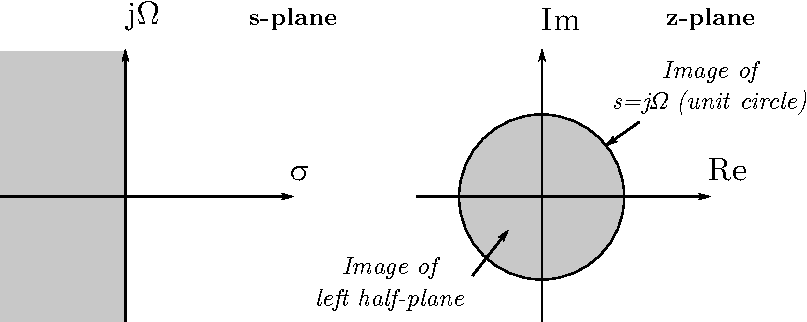
\includegraphics[width=0.6\textwidth]{figures/IIR_s2zBil}
\caption{Mapping the s-plane into z-domain.}
\label{fig:IIR_s2zBil}
\end{figure}

Because of the non-linear relation between the imaginary axis in continuous-time and dicrete-time, frequency warping (pre-warping) must be applied. If the requirements for the filter are derived in discrete-time the frequencies must be frequency warped such that the corresponding frequency in continuous-time is achieved. This is done by using \autoref{eq:frequencyRelationS2Z}. A comparison between bilinear transform and impulse invariant method is seen in \autoref{fig:IIR_transforms}. 


\begin{figure}[H]
\centering
\begin{subfigure}[t]{0.435\textwidth}
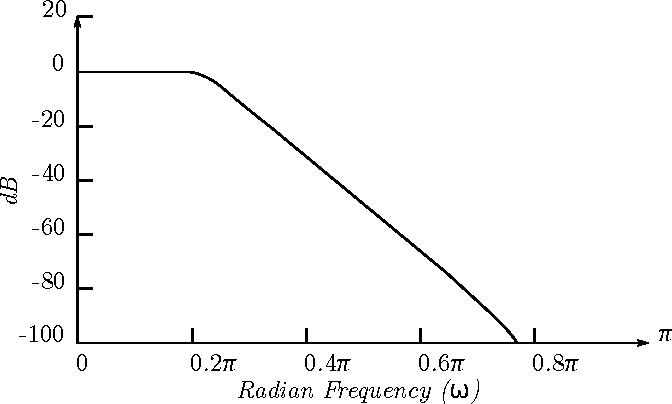
\includegraphics[width=\linewidth]{IIR_bil}
	\caption{Frequency response of system in z-domain by using bilinear transformation.}
	\label{fig:IIR_bil}
\end{subfigure}
\hspace{6mm} 
\begin{subfigure}[t]{0.47\textwidth}
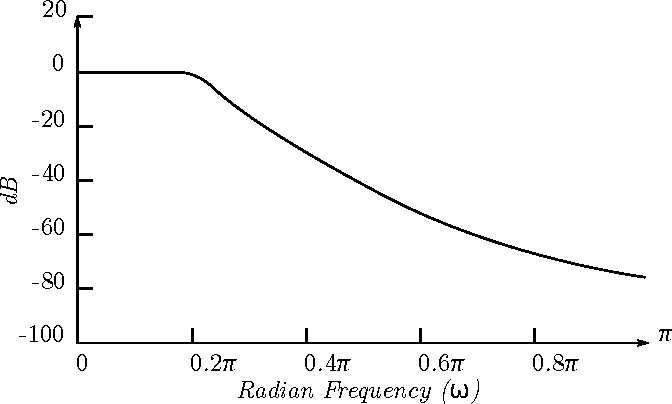
\includegraphics[width=\linewidth]{IIR_imp}
	\caption{Frequency response of system in z-domain by using impulse invariant method.}
	\label{fig:IIR_imp}
\end{subfigure}
\caption{Comparison of the frequency response by using bilinear transformation and impulse invariant method.}
\label{fig:IIR_transforms}
\end{figure}

Because the impulse invariant method imitates the frequency response of the analog filter, the consequence is aliasing if the attenuation at $\frac{f_s}{2}$ is not high enough. If the attenuation is high enough at $\frac{f_s}{2}$ e.g. -60 dB the aliasing may be neglected. By using bilinear transformation aliasing will not arise since the attenuation at $\pi$ in theory is $-\infty$. To apply the bilinear transform following expression is used:
\begin{align}
s = \frac{2}{T_s}\frac{z-1}{z+1}
\label{eq:bilinear_trans2}
\end{align}
All s-component is substituted with an expression consisting of z-component and is first used when the transfer function of the system in Laplace-domain is known. 

\section{Designing and implementing IIR filters}
There are many different types of filters that can be designed. Therefore this section will mainly focus on some of the methods and procedures that can be used to design an IIR filter. An example of designing a low-pass Butterworth filter is thus provided.

For a Butterworth filter the magnitude-squared function is given as:
\begin{align}
|H(j\Omega)|^2 = \frac{1}{1+(\frac{\Omega}{\Omega_c})^{2N}}
\label{eq:mag_sq}
\end{align}
From the requirements the order and cutoff frequency are determined. When the order is know the pole location can be determined. For a Butterworth filter, the pole location can be found with following expression.
\begin{align}
p_k = \Omega_c \cdot e^{\frac{j\pi}{2N}\cdot (2k+N-1)}, \quad k=0,1, ..., 2N-1
\label{eq:det_poles}
\end{align}
After the pole locations have been determined the transfer function for a Butterworth filter may be expressed as:
\begin{align}
H_c(s) = \frac{G}{\prod\limits_{k=1}^{N}(s-p_k)} 
\label{eq:trans_func_general}
\end{align}
The poles found in \autoref{eq:det_poles} are now inserted into \autoref{eq:trans_func_general}. To determine the gain, G, of the filter, the gain at DC i.e. $s=0$ is inserted into the equation. For a Butterworth filter the gain is $G=\Omega_c^N$, where $\Omega_c$ is the cutoff frequency and N is the order of the filter. After determining the transfer function a transformation is applied to transform the transfer function from s-domain into z-domain. After the transformation the transfer function is reduced into following form.
\begin{align}
H(z) = \frac{Y(z)}{X(z)} = \frac{\sum\limits_{k=0}^{M}b_kz^{-k}}{1 + \sum\limits_{k=1}^{N}a_kz^{-k}} 
\label{eq:trans_standard}
\end{align}
Where $b_k$ are coefficient for the zeros and $a_k$ are the coefficient for the poles and N and M are the order of the filter. In some literature the sign of the  coefficients $a_k$ are turned thus giving $1 - \sum\limits_{k=1}^{N}a_kz^{-k}$. In this example the signs of the $a_k$ coeffiecients are not turned, thus a plus instead of a minus.

To implement the digital filter the transfer function must be transformed back into discrete-time domain in order to implement it into CPU's such as microcontrollers and DSP's as they work in discrete-time domain. To do so, the inverse z-transformation is applied to the transfer function. \autoref{eq:trans_standard} is first rewritten into following:
\begin{align}
Y(z) = \sum\limits_{k=0}^{M}b_kz^{-k}X(z) -\sum\limits_{k=1}^{N}a_kz^{-k}Y(z)
\label{eq:z_domain_trans}
\end{align}
The time-shifting property is used as a part of the inverse z-transformation and is given as:
\begin{align}
x[n-k] \xleftrightarrow{Z} z^{-k} X(z)
\label{eq:time_shifting}
\end{align}
The inverse z-transformation is now applied and following difference equation is derived:
\begin{align}
y[n] =  \sum\limits_{k=0}^{M}b_kx[n-k] -\sum\limits_{k=1}^{N}a_ky[n-k]
\label{eq:time_domain2}
\end{align}
\autoref{eq:time_domain2} can then be implemented into a computer such as a DSP or microcontroller. Another topic is filter structures, which is a topic about how to implement filters efficiently. However since IIR-filters are not used in this project, no further discussion on the topic will be provided.










